\documentclass{beamer}
\usepackage[latin1]{inputenc}

\usepackage{graphicx}
\usepackage{listings}
\lstset{basicstyle=\tiny}

\newcommand{\bra}[1]{\langle #1|}
\newcommand{\ket}[1]{|#1\rangle}
\newcommand{\braket}[2]{\langle #1|#2\rangle}

\setlength{\parskip}{\baselineskip}

\usetheme{Warsaw}
\title[Valeev Group Meeting]{Valeev Group Meeting}
\author{Andrey Asadchev}
\institute{VT.edu}

\begin{document}

\begin{frame}
  \titlepage
\end{frame}

\begin{frame}{Picture of a goat!!!}
\begin{figure}[here]
\begin{center}
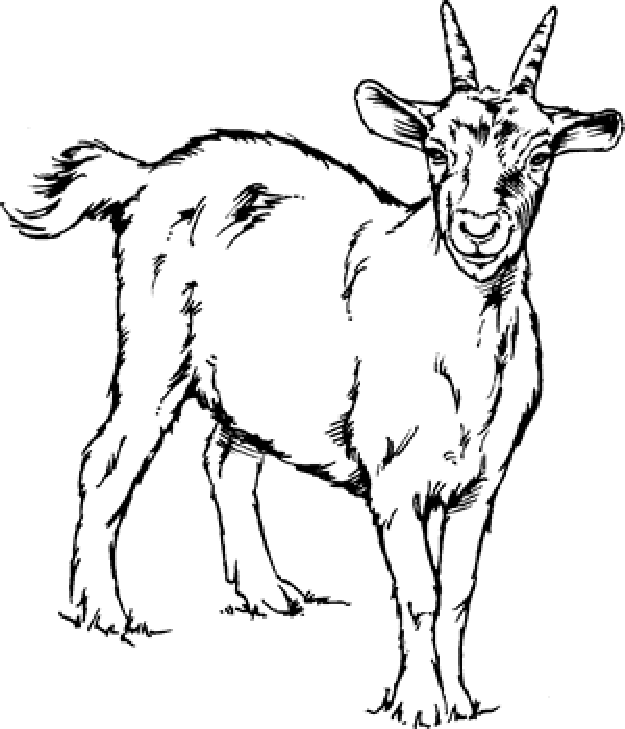
\includegraphics[scale=0.5]{goat.pdf}
\end{center}
\end{figure}
\end{frame}

\begin{frame}{Configuration Interaction on a conceptual level}
\begin{itemize}
\item Assume that we have $N_\alpha$ alpha electrons, $N_\beta$ beta electrons, and $K$ orbitals.
\item Then there are ${K \choose N_\alpha}$ alpha and ${K \choose N_\beta}$ arrangements.
\item Lets choose represent empty orbitals with 0s and occupied orbitals with 1s.
\item Then electron arrangements, called strings, can be represented as a {\it bit} string
\item For example $K = 4, N = 2$ configuration will generate $1100, 1010, 1001, 0110, 0101, 0011$
\item The number of strings grows quickly, $K = 32, N = 16$ will generate over 600 million strings.
\end{itemize}
\end{frame}

\begin{frame}{Configuration Interaction on a conceptual level}
\begin{itemize}
\item A determinant is an arrangement of alpha and beta electrons,
  which is really a pair of alpha and beta strings
\item Strings with all electrons occupying the lowest orbitals, ie the reference string,
  can be (arbitrarily) chosen to be $11..00$ and any other strings are said to be excited.
\item Similarly, the determinants are either reference or (singly, doubly, ...) excited.
\item CI expression $\ket{\Psi} = c_0 \bra{\Phi_0} + \sum{c_i^a \bra{\Phi_i^a} } +  ..$
 implemented in terms of determinants is called determinant CI.
\item There are other types of CI but the determinant CI has a huge computational advantage ...
\end{itemize}
\end{frame}

\begin{frame}{Determinant CI}
\begin{itemize}
\item There are ${K \choose N_\alpha}$ alpha and ${K \choose N_\beta}$ beta strings.
\item In Full CI there are then ${K \choose N_\alpha} {K \choose N_\alpha}$ determinants.
\item But the entire Hamiltonian is square the number of determinants!!!
\item Only for smallest of spaces can the Hamiltonian be evaluated in full and diagonalized.
\item For anything larger, the CI roots (eigenvalues) and coefficient vectors (CI vectors)
  need to be evaluated iteratively.
\item To do that fast, various Hamiltonian elements, eg
  $\bra{I_\alpha I_\beta} H \ket{J_\alpha J_\beta}$,
  need to be evaluated on the fly, fast. 
\item With determinant CI evaluation of those element can be fast.
\end{itemize}
\end{frame}

\begin{frame}{The three CI parts}
\begin{itemize}
\item The three types of CI excitations are alpha-alpha, beta-beta, and simultaneous alpha-beta.
\item Those are commonly referred to as $\sigma_1, \sigma_2, \sigma_3$. \\
\begin{align*}
\sigma_1(a,b) =& \sum_{b'} \sum_{ij}   { \bra{b} E_{ij}^{\beta} \ket{b'} h'_{ij} C(a,b') } + \\
& \sum_{b'} \sum_{ijkl} { \bra{b} E_{ij}^{\beta} \ket{b'} \bra{b} E_{kl}^{\beta} \ket{b'} (ij|kl) C(a,b') }
\\
\sigma_2(a,b) =&
  \sum_{a'} \sum_{ij}   { \bra{a} E_{ij}^{\alpha} \ket{a'} h'_{ij} C(a',b) } + \\
& \sum_{a'} \sum_{ijkl} { \bra{a} E_{ij}^{\alpha} \ket{a'} \bra{a} E_{kl}^{\alpha} \ket{a'} (ij|kl) C(a',b) }
 \\
\sigma_3(a,b) =& \sum_{a'b'} \sum_{ijkl} {
  \bra{a} E_{ij}^{\alpha} \ket{a'} \bra{b} E_{kl}^{\beta} \ket{b'} (ij|kl) C(a',b')
}
\end{align*}
\end{itemize}
\end{frame}

\begin{frame}{The three CI parts}
\begin{itemize}
\item In a nutshell, each string has a set of allowed excitation and with it associated a phase,
  string position in the list, and the integral indices.
\item I'll use notation $E^{aa'}_{ij}$ to signify allowed excitation from $a$ to $a'$,
  integral indices $i,j$ and the phase (1 or -1)
\item We want to make sure computing those elements is reasonably fast.
\end{itemize}
\end{frame}


\begin{frame}{CI String representation}
\begin{itemize}
\item Generally, a string of K orbitals can be represented using a K-bit integer.
\item This is an example of a {\em perfect} hash - each string is mapped to a unique number.
\item However raw integer mapping is not a {\em minimal} hash - there are lots of gaps.
\item What is desired is a {\em minimal perfect} hash s.t. all strings are mapped to a continuous integer range we can use for addressing.
\end{itemize}
\end{frame}

\begin{frame}{CI String hashing}
\begin{itemize}
\item For now we shall assume that we are dealing with at most 32 orbital strings.
\item Generate all valid strings in lexicographical order.
\item Observe that there are fast-changing (upper) and slow-changing (lower) halves.
\item Furthermore observe that upper half are the same for any given lower half.
\item Then we can construct a hash that uses upper half to lookup displacement of its lower half
 and the lower half to lookup the final index.
\item For a 32-bit string that requires two lookup tables , $2^{16}$ elements each (512kb).
\item {\tt hash(s) = U[16 >> s] + L[0xFFFF  \& s]}
\end{itemize}
\end{frame}

\begin{frame}[fragile]{CI String example}
\begin{verbatim}
std::vector<int> O, E(1); // reserve k->k excitation
for (int l = 0; l < I.size(); ++l) {
    if (I[l]) O.push_back(l); // occ. orbs
    if (!I[l]) E.push_back(l); // exc. orbs
}
for (auto o = O.begin(); o < O.end(); ++o) {
    int k = *o;
    E[0] = k; // k->k
    for (auto e = E.begin(); e < E.end(); ++e) {
        int l = *e;
        String J = I.swap(k, l);
        if (!ci.test(J,S)) continue;
        double sgn_kl = sgn(I, k, l);
        int kl = index(k, l);
        ...
\end{verbatim}
\end{frame}

\begin{frame}{CI String manipulations}
\begin{itemize}
\item Use {\tt std::bitset} and all its goodness
\item Swap two indices $i,j$: \\
  {\tt bitset.flip(i); bitset.flip(j); }
\item Compute phase of $i,j, i < j$: \\
  clear hi bits: {\tt s = s \& ((1<<j)-1) } \\
  clear lo bits: {\tt s = s >> i; s = s >> 1; } \\
  compute set bits: {\tt p = biset(s).count() OR \_mm\_popcnt(s) } \\
  even phase is 1, odd is -1: \\
  {\tt return (ij \% 2) ? -1 : 1; }
\item Test if the CI determinant is allowed.  Whaaaa .. ?
\end{itemize}
\end{frame}

\begin{frame}{Restricted CI}
\begin{itemize}
\item Number of the determinants can be reduced by dropping some.
\item In restricted CI, the determinants differing from reference by some factor are dropped.
\item For example in (4 4) CISD, determinant pair (1100,1010) is allowed but (0110,0011) is not.
\item To get the excitation of a string from reference, we need string distance.
\item With bit strings, it is easy by XOR string with reference: \\
  {\tt bitset(r \string^ s).count()/2; }
\item And total rank/excitation is the sum of alpha and beta rank/excitations
\end{itemize}
\end{frame}

\begin{frame}{Overall CI algorithm}
\begin{itemize}
\item CI algorithm can be broken down into two parts:  \\
  the calculation of $\sigma$ vector, $\sigma = \mathbf{H} c$ and Davidson iteration
\item $\sigma$ computation is computationally and I/O heavy, especially $\sigma_3$ part
\item The Davidson step is a straightforward linear algebra, primarily dot products and scaling.
\end{itemize}
\end{frame}

\begin{frame}{Sigma 1/2}
\begin{itemize}
\item Sigma 2 computations can be formulated as
  $\sigma(a,b) = \sum_{b'} F(b \rightarrow b') C(a,b')$, where $F(b \rightarrow b')$
  depends only on beta string excitation and corresponding one- and two- electron integrals.
  Sigma 1 for $a'$ is defined similarly
\item In the closed-shell case, $C(a,b)$ is symmetric and $\sigma_1(a,b) = -1^{S} \sigma_2(b,a)$
\item The expression can be rewritten as $\sigma(b,a) = \sum_{b'} F(b \rightarrow b') C(b',a)$
\item In other words, to compute column $a$ of $\sigma$, we only need the corresponding $C$ column
\item Very easy to parallelize and to distribute data, \\
  distribute data column-wise and operate on local columns of $C$ and $\sigma$
\item In case of open-shell, transpose either matrix/vector between the two steps
\end{itemize}
\end{frame}

\begin{frame}{Code-level optimization}
\begin{itemize}
\item Each processor has theoretical peak of performing operations,
  in our case floating-point operations.
\item For the purposes of chemistry we use double precision (8-byte/64-bit) floating point numbers (versus 4-byte single precision numbers.
\item We can know the peak performance of double precision operations if we know Instructions Per Cycle (IPC) rate. With modern x86-64 processors, double precision IPC is 4.
\item We then multiply IPC by processor frequency to get the Floating Operations Per Second (FLOPs). 
\end{itemize}
\end{frame}

\begin{frame}[fragile]{Code-level optimization}
\begin{itemize}
\item One of the biggest direct factors affecting IPC are
  Single Instruction Multiple Data (SIMD) instructions, also called vector instructions.
\item Vector instructions apply the same operator (eg multiply, add) to a {\tt vector} of operands
\item SSE vector length is 128 bits, AVX is 256 bits. \\
  128 bit SIMD can evaluate two sets of 64-bit operands for the price of one.
\item To make use of SIMD instructions, code must operate on contiguous chunks of data, eg: \\
\begin{verbatim}
for (int i = 0; i < N; ++i) {
    sigma[i] = f*C[i];
}
\end{verbatim}
\end{itemize}
\end{frame}

\begin{frame}[fragile]{Indirect addressing}
\begin{itemize}

\item Any sort of indirect addressing will kill code vectorization, eg:
\begin{verbatim}
for (int i = 0; i < N; ++i) {
    sigma[i] = f*C[index[i]];
}
\end{verbatim}
\item Guess what a naive CI kernel looks like?
\item One solution is to transpose data
\item Another solution is to factor out loops with indirect addressing
  and apply computed results in a loop with direct addressing.
\item Yet another solution is to reorder data to avoid indirect addressing
\item Or combination thereof!
\end{itemize}
\end{frame}

\begin{frame}[fragile]{Aliasing}
\begin{itemize}

\item Other factor that kills vectorization is pointer aliasing, eg:
\begin{verbatim}
double *sigma = ...;
const double *C = ...; 
for (int i = 0; i < N; ++i) {
    // compiler must assume sigma might point to C!!!
    sigma[i] = f*C[i];
}
\end{verbatim}

\item Solution is to tell compiler the pointer is not ``connected'' to other pointers
\begin{verbatim}
double *__restrict__ sigma = ...;
const double *__restrict__ C = ...; 
for (int i = 0; i < N; ++i) {
    sigma[i] = f*C[i];
}
\end{verbatim}
 
\end{itemize}
\end{frame}

\begin{frame}[fragile]{Sigma revisited}
  Recall in $\sigma(a,b) = \sum_{a'} F(a \rightarrow a') C(a',b)$, 
  $F(b \rightarrow a')$ depends only on alpha string and corresponding one- and two- electron integrals.
\begin{verbatim}
range rb = ...; // some beta subrange 
Matrix c = C(alpha, rb).transpose();
Matrix s(rb.size, alpha.size());
for (int i = 0; i < alpha.size(); ++i) {
    Vector F = Vector::Zero(alpha.size());
    // all excitation from alpha[i]
    F = sigma2(alpha[i], alpha, H, V);
    for (int k = 0; k < alpha.size(); ++k) {
        double f = F(k);
        if (fabs(f) < 1e-14) continue;
        s.col(i) += f*c.col(k);
    }
}
\end{verbatim}
\end{frame}

\begin{frame}[fragile]{Sigma 3}
\begin{itemize}
\item $\sigma_3(a,b) = \sum_{a'b'} F(a \rightarrow a', b \rightarrow b') C(a',b')$, 
\item Notice the big difference from earlier $\sigma$,
  neither rows nor columns ``match'' between $\sigma$ and $C$.
  That means a lot of I/O.
\item Lets say we need to compute a beta column $111000$.  Allowed excitations are  \\
$111000, 110100, 110010, 110001, 101100, ...$. \\
All those columns will need to be loaded.
\item What about a beta column $110100$?  Allowed excitations are \\
$111000, 110100, 110010, 110001, 101100, ...$. \\
That's a lot of overlap with a beta column $111000$.
\item I/O overhead can be hidden by computing a block of beta columns at a time.
\end{itemize}
\end{frame}

\begin{frame}[fragile]{Sigma 3}
 The general approach I took is as follows
\begin{itemize}
\item Pick a block of beta columns to compute.
\item For each of those beta strings, generate all valid excitations.
\item Sort excitation list
\item Loop over excitation list in blocks (list may have gaps)
\item Load $C(:,b')$ corresponding to that block
\item Evaluate $\sigma(:,b)$ columns corresponding to $C(:,b')$ block. \\
  Those $\sigma(:,b)$ columns aren't necessarily contiguous!
\item Now that I/O part is (kinda) taken care of, what about computational efficiency?
\end{itemize}
\end{frame}

\begin{frame}[fragile]{Sigma 3}
  There is a lot of indexing involved in 
  $\sigma_3(a,b) = \sum_{a',b'} E_{ij}^{aa'} E_{kl}^{bb'} (ij|kl) C(a',b')$ \\
  We need to get valid excitations, phase factors, orbitals that are swapped, etc.
  Lets try a few tricks.
\begin{itemize}
\item Make a subcopy of $(ij|kl)$, lets call it $(ij|b')$, corresponding to
  $b \rightarrow b'$ excitations in the block.
\item Apply $b \rightarrow b'$ phase factors to $(ij|b')$.
\item Now the $b'$ dimension no longer requires indirect indexing: \\
  $\sigma_3(a,b) = \sum_{a',b'} E_{ij}^{aa'} (ij|b') C(a',b')$.
\item Assuming column-major storage, need to transpose matrices.
\item There is no way to get rid of alpha indexing but
  for each alpha phase/index lookup there will be a block of vectorizable operations.
\end{itemize}
\end{frame}


\begin{frame}[fragile]{Performance}
Sample computation, 124,408,576,656 determinants, 64 nodes x 16 cores, 1024 total cores.
\begin{itemize}
\item Overall $\sigma$ time about 4300s, a bit over an hour.
\item $\sigma_{1+2}$ takes about 1300s
\item Out of that, $\sigma_{1+2}$ {\em kernel} accounts for about 50\%. Runs at about 20\% of peak.
\item $\sigma_{1+2}$ I/O (read and write) is about 10\%.
\item $\sigma_{3}$ takes about 3000s
\item Out of that, the {\em kernel} accounts for about two thirds of time.
\item I/O overhead isn't bad, on the order of 10\% but {\em data reordering} is rather expensive
\item With one-two expansion vectors, Davidson overhead is low, around 10\% of total wall time.
  Davidson wall time increases with the number of expansion vectors.
\end{itemize}
\end{frame}


\begin{frame}[fragile]{Current improvements}
Lexicographical ordering isn't the best.
\begin{itemize}
\item Consider the case of $\sigma_3$, for a rank $R$ string, only $R-1, R, R+1$ subset is needed.
\item With lexicographical ordering, the ranks are all over the place.
\item I/O is less localized {\em and} restricted CI is difficult to integrate.
\item Instead, (stable) sort the lexicographically ordered strings by their ranks.
\item Modify the loops to iterate over the blocks of excitation subspaces.
\item Improved data locality, integrating restricted CI is straightforward.
\item Slight overhead to string indexing:  the hash must assume lexicographical order.
\end{itemize}
\end{frame}


\begin{frame}[fragile]{Questions?}
Questions?
\begin{figure}[here]
\begin{center}
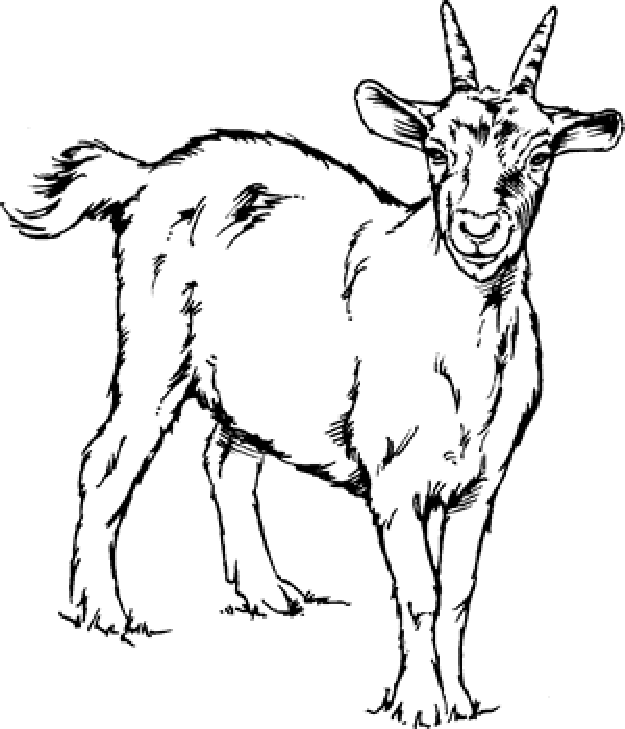
\includegraphics[scale=0.5]{goat.pdf}
\end{center}
\end{figure}
\end{frame}


\end{document}
